% ============================================================
% 讲义 — 人教版高一必修2 · 第10章 概率
% 编译命令：xelatex -interaction=nonstopmode 文件名.tex
% ============================================================
\documentclass[12pt, a4paper]{ctexart}
\usepackage[margin=2.2cm]{geometry}
\usepackage{amsmath, amssymb}
\usepackage{enumitem}
\usepackage{tcolorbox}
\usepackage{booktabs}
\usepackage{array}
\usepackage{fancyhdr}
\usepackage{xcolor}
\usepackage{tikz}
\usepackage{hyperref}
\usepackage{graphicx}
\usepackage{multirow}
\usepackage{pgfplots}
\pgfplotsset{compat=1.18}

% 颜色定义
\definecolor{mainblue}{RGB}{41, 98, 168}
\definecolor{lightblue}{RGB}{230, 240, 255}
\definecolor{tipgreen}{RGB}{34, 139, 87}
\definecolor{lightgreen}{RGB}{235, 250, 240}
\definecolor{warnred}{RGB}{200, 50, 50}
\definecolor{lightred}{RGB}{255, 240, 240}
\definecolor{examorange}{RGB}{210, 120, 20}
\definecolor{lightorange}{RGB}{255, 248, 235}
\definecolor{apppurple}{RGB}{120, 60, 170}
\definecolor{lightpurple}{RGB}{245, 238, 255}

% 页眉页脚
\pagestyle{fancy}
\fancyhf{}
\fancyhead[L]{\small\textcolor{mainblue}{\textbf{人教版高一必修2 · 第10章 概率}}}
\fancyhead[R]{\small\textcolor{mainblue}{概率论讲义}}
\fancyfoot[C]{\small —\ \thepage\ —}
\renewcommand{\headrulewidth}{0.6pt}
\renewcommand{\headrule}{\hbox to\headwidth{\color{mainblue}\leaders\hrule height \headrulewidth\hfill}}
\renewcommand{\footrulewidth}{0pt}

% tcolorbox 样式
\newtcolorbox{knowledgebox}[1][]{%
  colback=lightblue, colframe=mainblue,
  fonttitle=\bfseries\large, title=#1,
  arc=3mm, boxrule=0.8pt,
  left=8pt, right=8pt, top=6pt, bottom=6pt
}

\newtcolorbox{tipbox}[1][]{%
  colback=lightgreen, colframe=tipgreen,
  fonttitle=\bfseries, title=#1,
  arc=2mm, boxrule=0.6pt,
  left=6pt, right=6pt, top=4pt, bottom=4pt
}

\newtcolorbox{warnbox}[1][]{%
  colback=lightred, colframe=warnred,
  fonttitle=\bfseries, title=#1,
  arc=2mm, boxrule=0.6pt,
  left=6pt, right=6pt, top=4pt, bottom=4pt
}

\newtcolorbox{examplebox}[1][]{%
  colback=lightorange, colframe=examorange,
  fonttitle=\bfseries, title=#1,
  arc=3mm, boxrule=0.8pt,
  left=8pt, right=8pt, top=6pt, bottom=6pt
}

\newtcolorbox{appbox}[1][]{%
  colback=lightpurple, colframe=apppurple,
  fonttitle=\bfseries, title=#1,
  arc=3mm, boxrule=0.8pt,
  left=8pt, right=8pt, top=6pt, bottom=6pt
}

\setCJKmainfont{Hiragino Sans GB}
\setCJKsansfont{Heiti SC}

\begin{document}

% ============ 标题页 ============
\begin{center}
{\Huge\bfseries\textcolor{mainblue}{第10章\quad 概\quad 率}}\\[12pt]
{\Large\textcolor{gray}{讲\quad 义}}\\[8pt]
\rule{0.6\textwidth}{1pt}\\[8pt]
{\normalsize 适用：人教版\quad 高一必修2\quad |\quad 课时：8课时}
\end{center}
\vspace{10pt}

% ================================================================
%  第一部分：知识点讲解
% ================================================================
\section*{\textcolor{mainblue}{一、知识点讲解}}

% ---- 10.1 随机事件 ----
\subsection*{10.1\quad 随机事件}

\begin{knowledgebox}[随机试验与随机事件]
\textbf{随机试验}满足三个条件：
\begin{enumerate}[label=(\arabic*)]
  \item 可以在相同条件下重复进行；
  \item 每次试验的可能结果不止一个，且能事先明确所有可能结果；
  \item 进行一次试验前不能确定哪个结果会出现。
\end{enumerate}

\textbf{随机事件}：在一定条件下可能发生也可能不发生的事件，用大写字母 $A, B, C, \ldots$ 表示。
\end{knowledgebox}

\begin{knowledgebox}[事件的分类]
\begin{itemize}
  \item \textbf{必然事件}：在条件 $S$ 下一定会发生的事件，记为 $\Omega$。
  \item \textbf{不可能事件}：在条件 $S$ 下一定不会发生的事件，记为 $\varnothing$。
  \item \textbf{随机事件}：可能发生也可能不发生的事件。
\end{itemize}
\end{knowledgebox}

\begin{knowledgebox}[频率与概率]
\textbf{频率}：在 $n$ 次重复试验中，事件 $A$ 发生了 $n_A$ 次，则 $\dfrac{n_A}{n}$ 称为事件 $A$ 的\textbf{频率}。

\textbf{概率}：随着试验次数增加，频率稳定在一个常数附近，这个常数称为事件 $A$ 的\textbf{概率}，记为 $P(A)$。

\textbf{性质}：
\begin{itemize}
  \item $0 \leqslant P(A) \leqslant 1$
  \item $P(\Omega) = 1$，$P(\varnothing) = 0$
\end{itemize}
\end{knowledgebox}

\begin{warnbox}[易错提醒]
\begin{itemize}
  \item 频率是试验的结果，会随试验变化；概率是客观常数。
  \item $P(A) = 0$ 不代表 $A$ 是不可能事件；$P(A) = 1$ 不代表 $A$ 是必然事件。
  \item 频率是概率的估计值，试验次数越多，频率越接近概率。
\end{itemize}
\end{warnbox}

% ---- 10.2 古典概型 ----
\subsection*{10.2\quad 古典概型}

\begin{knowledgebox}[古典概型的定义]
若随机试验满足：
\begin{enumerate}[label=(\arabic*)]
  \item \textbf{有限性}：所有可能结果只有有限个，$\Omega = \{\omega_1, \omega_2, \ldots, \omega_n\}$；
  \item \textbf{等可能性}：每个基本事件发生的概率相等；
\end{enumerate}
则称该试验为\textbf{古典概型}（等可能概型）。
\end{knowledgebox}

\begin{knowledgebox}[古典概型概率公式]
\[
P(A) = \frac{\text{事件 } A \text{ 包含的基本事件数}}{\text{基本事件总数}} = \frac{m}{n}
\]
\end{knowledgebox}

\begin{tipbox}[求古典概型概率的步骤]
\begin{enumerate}[label=(\arabic*)]
  \item 确定样本空间，列举所有等可能的基本事件；
  \item 确定事件 $A$ 包含哪些基本事件；
  \item 计算 $P(A) = \dfrac{m}{n}$。
\end{enumerate}
常用方法：列举法、树状图法、列表法。
\end{tipbox}

% ---- 10.3 几何概型 ----
\subsection*{10.3\quad 几何概型}

\begin{knowledgebox}[几何概型的定义]
若每个基本事件对应几何区域 $\Omega$ 中的一个点，事件 $A$ 对应子区域 $A$，且点落在 $A$ 内的概率只与 $A$ 的\textbf{度量}（长度、面积、体积）成正比，与位置和形状无关，则称该模型为\textbf{几何概型}。
\end{knowledgebox}

\begin{knowledgebox}[几何概型概率公式]
\[
P(A) = \frac{\text{事件 } A \text{ 对应区域的度量}}{\text{全部结果对应区域的度量}}
\]

度量可以是长度、面积或体积。
\end{knowledgebox}

\begin{warnbox}[古典概型与几何概型的比较]
\begin{itemize}
  \item 古典概型：样本空间有限，用\textbf{计数}求概率。
  \item 几何概型：样本空间无限（不可数），用\textbf{度量}求概率。
  \item 两者都要求"等可能性"。
\end{itemize}
\end{warnbox}

% ---- 10.4 概率的基本性质 ----
\subsection*{10.4\quad 概率的基本性质}

\begin{knowledgebox}[概率的基本性质]
\begin{enumerate}[label=(\arabic*)]
  \item \textbf{非负性}：对任意事件 $A$，$P(A) \geqslant 0$。
  \item \textbf{规范性}：$P(\Omega) = 1$。
  \item \textbf{可加性}：若 $A$ 与 $B$ 互斥，则 $P(A \cup B) = P(A) + P(B)$。
\end{enumerate}

推广：若 $A_1, A_2, \ldots, A_n$ 两两互斥，则
\[
P(A_1 \cup A_2 \cup \cdots \cup A_n) = P(A_1) + P(A_2) + \cdots + P(A_n)
\]
\end{knowledgebox}

\begin{knowledgebox}[一般加法公式（容斥原理）]
对任意两个事件 $A$ 与 $B$：
\[
P(A \cup B) = P(A) + P(B) - P(A \cap B)
\]

当 $A$ 与 $B$ 互斥时，$P(A \cap B) = 0$，退化为 $P(A \cup B) = P(A) + P(B)$。
\end{knowledgebox}

% ---- 10.5 互斥事件与对立事件 ----
\subsection*{10.5\quad 互斥事件与对立事件}

\begin{knowledgebox}[互斥事件]
若事件 $A$ 与事件 $B$ \textbf{不能同时发生}（即 $A \cap B = \varnothing$），则称 $A$ 与 $B$ 是\textbf{互斥事件}（互不相容事件）。

此时：$P(A \cup B) = P(A) + P(B)$。
\end{knowledgebox}

\begin{knowledgebox}[对立事件]
若事件 $A$ 与事件 $B$ 满足：
\begin{enumerate}[label=(\arabic*)]
  \item $A \cap B = \varnothing$（互斥）；
  \item $A \cup B = \Omega$（必有一个发生）；
\end{enumerate}
则称 $A$ 与 $B$ 互为\textbf{对立事件}，记 $B = \bar{A}$。

核心公式：$P(\bar{A}) = 1 - P(A)$。
\end{knowledgebox}

\begin{warnbox}[互斥与对立的关系]
\begin{itemize}
  \item 对立 $\Longrightarrow$ 互斥，但互斥 $\not\!\!\Longrightarrow$ 对立。
  \item 对立是特殊的互斥：两个事件合起来恰好覆盖整个样本空间。
  \item "正难则反"：求"至少一个"的概率时，用对立事件通常更简便。
\end{itemize}
\end{warnbox}

\begin{tipbox}[概率计算常用技巧]
\begin{itemize}
  \item 求"至少一个"的概率：$P(\text{至少一个}) = 1 - P(\text{一个也没有})$。
  \item 多个互斥事件的概率可以直接相加。
  \item 用加法公式前先判断是否互斥：互斥直接相加，非互斥需减去交集。
\end{itemize}
\end{tipbox}

% ================================================================
%  第二部分：例题精讲
% ================================================================
\section*{\textcolor{examorange}{二、例题精讲}}

\begin{examplebox}[【例1】古典概型——掷骰子]
同时掷两枚骰子，求点数之和为 $7$ 的概率。
\end{examplebox}

\textbf{解}：

样本空间：$(i, j)$，$i, j \in \{1,2,3,4,5,6\}$，共 $6 \times 6 = 36$ 个基本事件。

事件 $A$："点数之和为 $7$"，满足 $i + j = 7$ 的组合有：$(1,6),\ (2,5),\ (3,4),\ (4,3),\ (5,2),\ (6,1)$，共 $6$ 个。

\[
P(A) = \frac{6}{36} = \frac{1}{6}
\]

\begin{examplebox}[【例2】古典概型——摸球问题]
口袋中有 $3$ 个红球和 $2$ 个白球（除颜色外完全相同），不放回地依次摸出 $2$ 个球，求两个球颜色不同的概率。
\end{examplebox}

\textbf{解}：

从 $5$ 个球中不放回摸出 $2$ 个，用组合：$n = C_5^2 = 10$。

事件 $A$："一红一白"：$m = C_3^1 \times C_2^1 = 6$。

\[
P(A) = \frac{6}{10} = \frac{3}{5}
\]

\begin{examplebox}[【例3】几何概型——长度型]
在区间 $[0, 10]$ 上随机取一个数 $x$，求 $3 \leqslant x \leqslant 7$ 的概率。
\end{examplebox}

\textbf{解}：

总区域 $[0, 10]$ 的长度为 $10$，事件区域 $[3, 7]$ 的长度为 $4$。

\[
P = \frac{4}{10} = \frac{2}{5}
\]

\begin{examplebox}[【例4】几何概型——面积型]
边长为 $2$ 的正方形内有一个内切圆。向正方形内随机投一点，求该点落在圆内的概率。
\end{examplebox}

\textbf{解}：

正方形面积 $= 2^2 = 4$，内切圆半径 $r = 1$，圆面积 $= \pi$。

\[
P = \frac{\pi}{4} \approx 0.785
\]

\begin{center}
\begin{tikzpicture}[scale=1.2]
\draw[fill=lightblue, draw=mainblue, thick] (0,0) rectangle (2,2);
\draw[fill=lightgreen, draw=tipgreen, thick] (1,1) circle (1);
\node at (1, 2.3) {正方形};
\node at (1, -0.3) {内切圆};
\end{tikzpicture}
\end{center}

\begin{examplebox}[【例5】互斥与对立事件]
某射手射击一次，命中 $10$ 环概率 $0.2$，$9$ 环概率 $0.3$，$8$ 环概率 $0.3$，$7$ 环及以下概率 $0.2$。
(1) 求"命中 $9$ 环或 $10$ 环"的概率。(2) 求"至少命中 $8$ 环"的概率。
\end{examplebox}

\textbf{解}：

设 $A_i$ 为"命中 $i$ 环"，各事件两两互斥。

(1) $P(A_{10} \cup A_9) = 0.2 + 0.3 = 0.5$

(2) 方法一（直接相加）：$P = 0.2 + 0.3 + 0.3 = 0.8$

方法二（对立事件）：$P = 1 - P(\text{7环及以下}) = 1 - 0.2 = 0.8$

\begin{examplebox}[【例6】概率加法公式（容斥原理）]
从一副去掉大小王的 $52$ 张扑克牌中随机抽一张，求抽到红色牌（红心或方块）或人头牌（J/Q/K）的概率。
\end{examplebox}

\textbf{解}：

设 $A$："红色牌"，$B$："人头牌"。

\[
P(A) = \frac{26}{52} = \frac{1}{2}, \quad P(B) = \frac{12}{52} = \frac{3}{13}, \quad P(A \cap B) = \frac{6}{52} = \frac{3}{26}
\]

$A$ 与 $B$ 不互斥（红色人头牌存在），用容斥原理：
\[
P(A \cup B) = \frac{1}{2} + \frac{3}{13} - \frac{3}{26} = \frac{13+6-3}{26} = \frac{16}{26} = \frac{8}{13}
\]

\begin{examplebox}[【例7】古典概型——有放回抽样]
袋中有 $4$ 个红球和 $6$ 个白球，有放回地取 $2$ 次，每次取 $1$ 个。求两次都取到红球的概率。
\end{examplebox}

\textbf{解}：

有放回抽取，每次独立。样本空间：$10 \times 10 = 100$ 种。

事件 $A$："两次都红"：$4 \times 4 = 16$ 种。

\[
P(A) = \frac{16}{100} = \frac{4}{25}
\]

\begin{examplebox}[【例8】几何概型——面积综合]
在矩形区域 $[0, 4] \times [0, 3]$ 内随机取一点 $(x, y)$，求 $x + y \leqslant 3$ 的概率。
\end{examplebox}

\textbf{解}：

矩形面积 $= 4 \times 3 = 12$。

满足 $x + y \leqslant 3$ 且 $0 \leqslant x \leqslant 4$，$0 \leqslant y \leqslant 3$ 的区域是一个三角形（顶点为 $(0,0)$，$(3,0)$，$(0,3)$），面积 $= \dfrac{1}{2} \times 3 \times 3 = \dfrac{9}{2}$。

\[
P = \frac{9/2}{12} = \frac{9}{24} = \frac{3}{8}
\]

\begin{center}
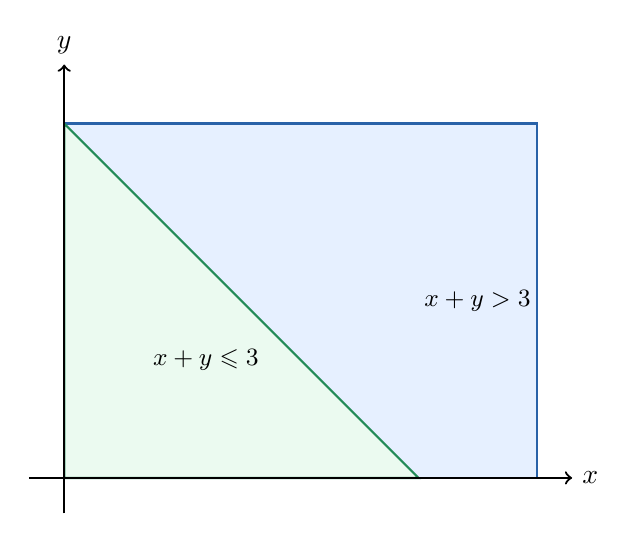
\begin{tikzpicture}[scale=1.5]
\draw[fill=lightblue, draw=mainblue, thick] (0,0) rectangle (4,3);
\draw[fill=lightgreen, draw=tipgreen, thick] (0,0) -- (3,0) -- (0,3) -- cycle;
\draw[->, thick] (-0.3,0) -- (4.3,0) node[right] {$x$};
\draw[->, thick] (0,-0.3) -- (0,3.5) node[above] {$y$};
\node at (1.2, 1) {\small $x+y \leqslant 3$};
\node at (3.5, 1.5) {\small $x+y > 3$};
\end{tikzpicture}
\end{center}

\begin{examplebox}[【例9】对立事件综合]
$3$ 人独立破译密码，各自能破译的概率分别为 $0.3,\ 0.4,\ 0.5$。求密码被破译的概率。
\end{examplebox}

\textbf{解}：

设 $A_i$ 为"第 $i$ 人能破译"。密码被破译 $=$ 至少有一人破译。

用对立事件：密码未被破译 $=$ 三人都未破译。

\[
P(\bar{A_1} \cap \bar{A_2} \cap \bar{A_3}) = (1-0.3)(1-0.4)(1-0.5) = 0.7 \times 0.6 \times 0.5 = 0.21
\]

\[
P(\text{被破译}) = 1 - 0.21 = 0.79
\]

\begin{examplebox}[【例10】概率综合——掷两枚骰子]
同时掷两枚骰子，求：(1) 点数之和为偶数的概率；(2) 至少一枚为 $6$ 的概率。
\end{examplebox}

\textbf{解}：

样本空间共 $36$ 个基本事件。

(1) 点数之和为偶数 $=$ 两数同奇或同偶。

奇数 $= \{1,3,5\}$，偶数 $= \{2,4,6\}$。

同奇：$3 \times 3 = 9$ 种；同偶：$3 \times 3 = 9$ 种。共 $18$ 种。

\[
P = \frac{18}{36} = \frac{1}{2}
\]

(2) 用对立事件："没有 $6$" $=$ 两枚都不是 $6$，共 $5 \times 5 = 25$ 种。

\[
P = 1 - \frac{25}{36} = \frac{11}{36}
\]

% ================================================================
%  第三部分：应用题
% ================================================================
\section*{\textcolor{apppurple}{三、应用题}}

\begin{appbox}[【应用1】商场抽奖]
某商场抽奖箱中有 $100$ 张奖券：一等奖 $1$ 张，二等奖 $3$ 张，三等奖 $6$ 张。随机抽一张。
(1) 求中奖概率。(2) 求中一等奖或二等奖的概率。(3) 求不中三等奖的概率。
\end{appbox}

\textbf{解}：

(1) 中奖 $= 1 + 3 + 6 = 10$ 张。$P(\text{中奖}) = \dfrac{10}{100} = \dfrac{1}{10}$

(2) 一等或二等奖共 $4$ 张。$P = \dfrac{4}{100} = \dfrac{1}{25}$

(3) 对立事件：$P = 1 - \dfrac{6}{100} = \dfrac{94}{100} = \dfrac{47}{50}$

\begin{appbox}[【应用2】公交候车问题]
公交车每 $10$ 分钟发一辆，乘客随机到达车站。求候车时间不超过 $3$ 分钟的概率。
\end{appbox}

\textbf{解}：

乘客在 $[0, 10)$ 内随机到达，设距上一班车发出 $x$ 分钟。

候车不超过 $3$ 分钟 $=$ 在上一班车发出后 $7 \sim 10$ 分钟到达：$x \in [7, 10)$。

\[
P = \frac{10 - 7}{10} = \frac{3}{10}
\]

\begin{appbox}[【应用3】天气预报与概率]
某地 $7$ 月晴天概率 $0.5$，多云概率 $0.3$，雨天概率 $0.2$。
(1) 求某天不是雨天的概率。(2) 求某天是晴天或多云的概率。(3) 若连续两天独立，求两天都下雨的概率。
\end{appbox}

\textbf{解}：

设 $A$："晴天"，$B$："多云"，$C$："雨天"，三者两两互斥且 $A \cup B \cup C = \Omega$。

(1) $P(\text{不是雨天}) = 1 - P(C) = 1 - 0.2 = 0.8$

(2) $P(A \cup B) = P(A) + P(B) = 0.5 + 0.3 = 0.8$

(3) 两天独立：$P(\text{都下雨}) = P(C) \times P(C) = 0.2 \times 0.2 = 0.04$

\begin{center}
\begin{tikzpicture}
\begin{axis}[
    ybar,
    width=8cm, height=5.5cm,
    xlabel={天气类型},
    ylabel={概率},
    ymin=0, ymax=0.6,
    xtick={1,2,3},
    xticklabels={晴天, 多云, 雨天},
    bar width=1.5cm,
    fill=lightblue,
    draw=mainblue,
    nodes near coords,
    every node near coord/.append style={font=\bfseries},
    axis lines=left,
]
\addplot[fill=lightblue, draw=mainblue] coordinates {
    (1, 0.5) (2, 0.3) (3, 0.2)
};
\end{axis}
\end{tikzpicture}
\end{center}

% ================================================================
%  第四部分：课堂练习
% ================================================================
\section*{\textcolor{tipgreen}{四、课堂练习}}

\begin{enumerate}
  \item 从 $1, 2, 3, 4, 5$ 中随机取一个数，求取到偶数的概率。

  \item 同时掷两枚硬币，求至少一枚正面朝上的概率。

  \item 在区间 $[0, 20]$ 上随机取一个数 $x$，求 $x > 12$ 的概率。

  \item 袋中有 $4$ 红球和 $6$ 白球，任取一个，求取到红球的概率。

  \item 已知 $P(A) = 0.4$，$P(B) = 0.5$，$A$ 与 $B$ 互斥，求 $P(A \cup B)$。

  \item 正方形边长为 $4$，内切圆半径为 $2$。随机投一点，求落在圆外的概率。

  \item 袋中有 $3$ 红球和 $2$ 白球，不放回摸出 $2$ 个，求至少一个红球的概率。

  \item 某人射击命中率 $0.7$，射击 $2$ 次（独立），求至少命中一次的概率。
\end{enumerate}

\begin{knowledgebox}[参考答案]
\begin{enumerate}
  \item 偶数有 $2, 4$，$P = \dfrac{2}{5}$。

  \item 样本空间 $\{(\text{正,正}),(\text{正,反}),(\text{反,正}),(\text{反,反})\}$。$P = \dfrac{3}{4}$。或用对立：$P = 1 - \dfrac{1}{4} = \dfrac{3}{4}$。

  \item $x > 12$ 的区间长度 $= 8$。$P = \dfrac{8}{20} = \dfrac{2}{5}$。

  \item $P = \dfrac{4}{10} = \dfrac{2}{5}$。

  \item $A$ 与 $B$ 互斥：$P(A \cup B) = 0.4 + 0.5 = 0.9$。

  \item 正方形面积 $= 16$，圆面积 $= 4\pi$。$P = \dfrac{16 - 4\pi}{16} = 1 - \dfrac{\pi}{4} \approx 0.215$。

  \item 对立事件：$P(\text{两个都白}) = \dfrac{C_2^2}{C_5^2} = \dfrac{1}{10}$。$P(\text{至少一个红}) = 1 - \dfrac{1}{10} = \dfrac{9}{10}$。

  \item 对立事件：$P(\text{都没中}) = 0.3 \times 0.3 = 0.09$。$P(\text{至少一次}) = 1 - 0.09 = 0.91$。
\end{enumerate}
\end{knowledgebox}

\vfill
\begin{center}
\small\textcolor{gray}{本讲义仅供教学参考，例题可根据学生水平调整难度。}
\end{center}

\end{document}
